\documentclass[11pt]{article} 
\usepackage{calc}
\usepackage[margin={1in,1in}]{geometry} 
\usepackage[hwkhandout]{hwk}
\usepackage[pdftitle={Calc 1
  Notes},colorlinks=true,urlcolor=blue]{hyperref}
\usepackage{tikz}

\renewcommand{\theclass}{\textsc{math}1300: calculus I}
\renewcommand{\theauthor}{Tyson Gern}
\renewcommand{\theassignment}{Related Rates}
\renewcommand{\dateinfo}{section 4.6}

\newcommand{\ds}{\displaystyle}

\begin{document}
\drawtitle

\noindent \textbf{Remember to draw pictures!}

\begin{enumerate}
\item A spherical snowball is melting. Its radius is decreasing at 0.2
  cm per hour when the radius is 15cm. How fast is its volume
  decreasing at that time? (The volume $V$ of a sphere of radius $r$
  is given by $V=\frac{4}{3}\pi r^3$)

  \newpage

\item A tank of water in the shape of a cone is leaking water at a
  constant rate of 2 cubic feet per hour. The radius of the top of the
  tank is 5 feet and the height of the tank is 14 feet. At what rate
  is the depth of the water in the tank changing when the depth of the
  water is 6 ft? (The volume $V$ of a cone of radius $r$ and height
  $h$ is given by $V=\frac{1}{3}\pi r^2 h$)

  \newpage

\item Two people on bikes start riding from the same position.  Person
  A starts riding north at a rate of 20 miles per hour. Person B starts
  riding east at 25 miles per hour.  At what rate is the distance
  separating the two people changing after 3 hours?
  

  \newpage

\item A lighthouse is 1 km offshore, and rotates clockwise once every
  minute.  When the angle $\theta=\dfrac{\pi}{6}$ (see diagram below),
  how fast is the beam of light moving along the shoreline in
  kilometers per hour?
  \begin{center}
    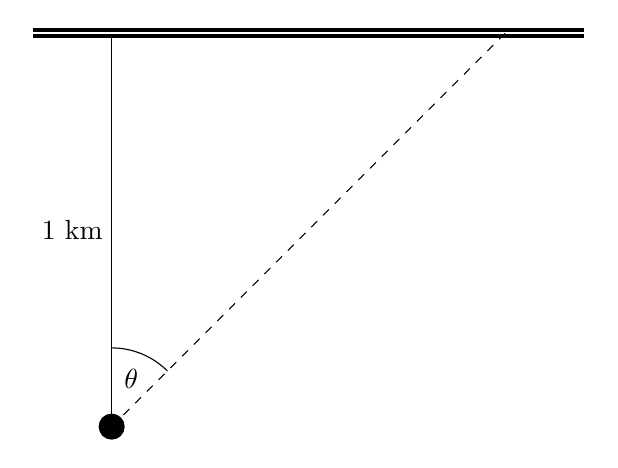
\begin{tikzpicture}[scale=1]
      \draw[<->] (1,5) -- (1,0);
      \draw[double, ultra thick](0,5)--(7,5);
      \draw[dashed] (1,0) -- (6,5);
      \node at (.5, 2.5) {1 km};
      \node[circle, fill=black] at (1,0) {};
      \draw (1,1) arc(90:45:1);
      \node at (1.25, .6) {$\theta$};
    \end{tikzpicture}
  \end{center}

\end{enumerate}

\end{document}
